\paragraph{QuizziPedia::Front-End::Directives::MenuBarDirective}

\label{QuizziPedia::Front-End::Directives::MenuBarDirective}

\begin{figure}[h]
	\centering
	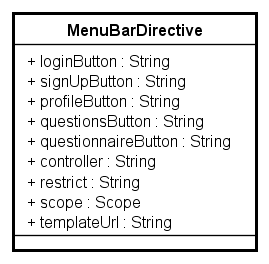
\includegraphics[scale=0.5,keepaspectratio]{UML/Classi/Front-End/QuizziPedia_Front-end_Directives_MenuBarDirective.png}
	\caption{QuizziPedia::Front-End::Directives::MenuBarDirective}
\end{figure}

\begin{itemize}
	\item \textbf{Descrizione}: ;
	\item \textbf{Utilizzo}: ;
	\item \textbf{Relazioni con altre classi}: 
	\begin{itemize}
		\item \textit{IN} \texttt{}: 
	\end{itemize}
	\item \textbf{Attributi}: 
	\begin{itemize}
		\item ;
	\end{itemize}
	\item \textbf{Metodi}: 
	\begin{itemize}
		\item ;
	\end{itemize}
\end{itemize}

\paragraph{QuizziPedia::Front-End::Directives::NewQuestionButtonDirective}

\label{QuizziPedia::Front-End::Directives::NewQuestionButtonDirective}

\begin{figure}[h]
	\centering
	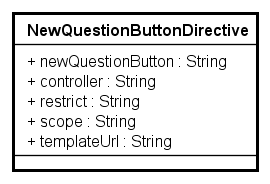
\includegraphics[scale=0.5,keepaspectratio]{UML/Classi/Front-End/QuizziPedia_Front-end_Directives_NewQuestionButtonDirective.png}
	\caption{QuizziPedia::Front-End::Directives::NewQuestionButtonDirective}
\end{figure}

\begin{itemize}
	\item \textbf{Descrizione}: ;
	\item \textbf{Utilizzo}: ;
	\item \textbf{Relazioni con altre classi}: 
	\begin{itemize}
		\item \textit{IN} \texttt{}: 
	\end{itemize}
	\item \textbf{Attributi}: 
	\begin{itemize}
		\item ;
	\end{itemize}
	\item \textbf{Metodi}: 
	\begin{itemize}
		\item ;
	\end{itemize}
\end{itemize}

\paragraph{QuizziPedia::Front-End::Directives::OneQuestionDirective}

\label{QuizziPedia::Front-End::Directives::OneQuestionDirective}

\begin{figure}[h]
	\centering
	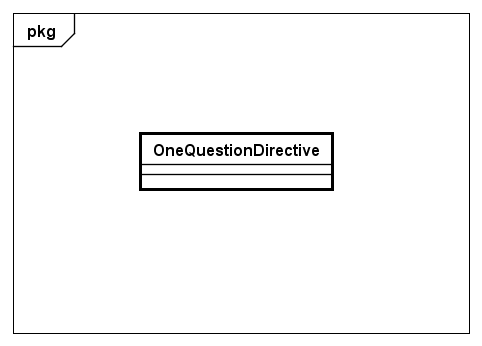
\includegraphics[scale=0.5,keepaspectratio]{UML/Classi/Front-End/QuizziPedia_Front-end_Directives_OneQuestionDirective.png}
	\caption{QuizziPedia::Front-End::Directives::OneQuestionDirective}
\end{figure}

\begin{itemize}
	\item \textbf{Descrizione}: ;
	\item \textbf{Utilizzo}: ;
	\item \textbf{Relazioni con altre classi}: 
	\begin{itemize}
		\item \textit{IN} \texttt{}: 
	\end{itemize}
	\item \textbf{Attributi}: 
	\begin{itemize}
		\item ;
	\end{itemize}
	\item \textbf{Metodi}: 
	\begin{itemize}
		\item ;
	\end{itemize}
\end{itemize}

\paragraph{QuizziPedia::Front-End::Directives::QuestionTextDirective}

\label{QuizziPedia::Front-End::Directives::QuestionTextDirective}

\begin{figure}[h]
	\centering
	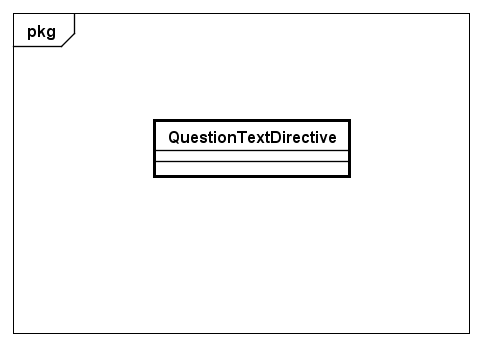
\includegraphics[scale=0.5,keepaspectratio]{UML/Classi/Front-End/QuizziPedia_Front-end_Directives_QuestionTextDirective.png}
	\caption{QuizziPedia::Front-End::Directives::QuestionTextDirective}
\end{figure}

\begin{itemize}
	\item \textbf{Descrizione}: ;
	\item \textbf{Utilizzo}: ;
	\item \textbf{Relazioni con altre classi}: 
	\begin{itemize}
		\item \textit{IN} \texttt{}: 
	\end{itemize}
	\item \textbf{Attributi}: 
	\begin{itemize}
		\item ;
	\end{itemize}
	\item \textbf{Metodi}: 
	\begin{itemize}
		\item ;
	\end{itemize}
\end{itemize}

\paragraph{QuizziPedia::Front-End::Directives::QuestionnaireDetailsDirective}

\label{QuizziPedia::Front-End::Directives::QuestionnaireDetailsDirective}

\begin{figure}[h]
	\centering
	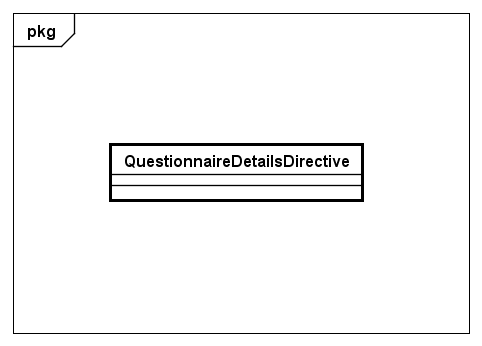
\includegraphics[scale=0.5,keepaspectratio]{UML/Classi/Front-End/QuizziPedia_Front-end_Directives_QuestionnaireDetailsDirective.png}
	\caption{QuizziPedia::Front-End::Directives::QuestionnaireDetailsDirective}
\end{figure}

\begin{itemize}
	\item \textbf{Descrizione}: ;
	\item \textbf{Utilizzo}: ;
	\item \textbf{Relazioni con altre classi}: 
	\begin{itemize}
		\item \textit{IN} \texttt{}: 
	\end{itemize}
	\item \textbf{Attributi}: 
	\begin{itemize}
		\item ;
	\end{itemize}
	\item \textbf{Metodi}: 
	\begin{itemize}
		\item ;
	\end{itemize}
\end{itemize}

\paragraph{QuizziPedia::Front-End::Directives::QuestionsManagementQuestionnaireDirective}

\label{QuizziPedia::Front-End::Directives::QuestionsManagementQuestionnaireDirective}

\begin{figure}[h]
	\centering
	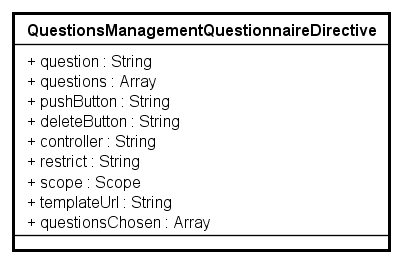
\includegraphics[scale=0.5,keepaspectratio]{UML/Classi/Front-End/QuizziPedia_Front-end_Directives_QuestionsManagementQuestionnaireDirective.png}
	\caption{QuizziPedia::Front-End::Directives::}
\end{figure}

\begin{itemize}
	\item \textbf{Descrizione}: ;
	\item \textbf{Utilizzo}: ;
	\item \textbf{Relazioni con altre classi}: 
	\begin{itemize}
		\item \textit{IN} \texttt{}: 
	\end{itemize}
	\item \textbf{Attributi}: 
	\begin{itemize}
		\item ;
	\end{itemize}
	\item \textbf{Metodi}: 
	\begin{itemize}
		\item ;
	\end{itemize}
\end{itemize}